%\section{Evaluation: Scalability of the Current Implementation}\label{sec:evaluation}
\section{Implementations}\label{sec:Implementation}

As edge and fog technologies are by many seen as additions to pure cloud approaches and most current factory implementations are using central clouds, many works are based on a mix between Edge and Cloud technologies. One such approach was introduced by Peralta et al in order to reduce the energy consumptions by the devices at the shop floor. Their approach is based on a three layered architecture, where those layers are composed of IoT nodes at the lowest level, an intermediate fog layer with IoT-Gateways and a cloud layer for crucial decision making and logging. An example of this architecture is shown in Fig. ???. 

\begin{figure}
	\centering
	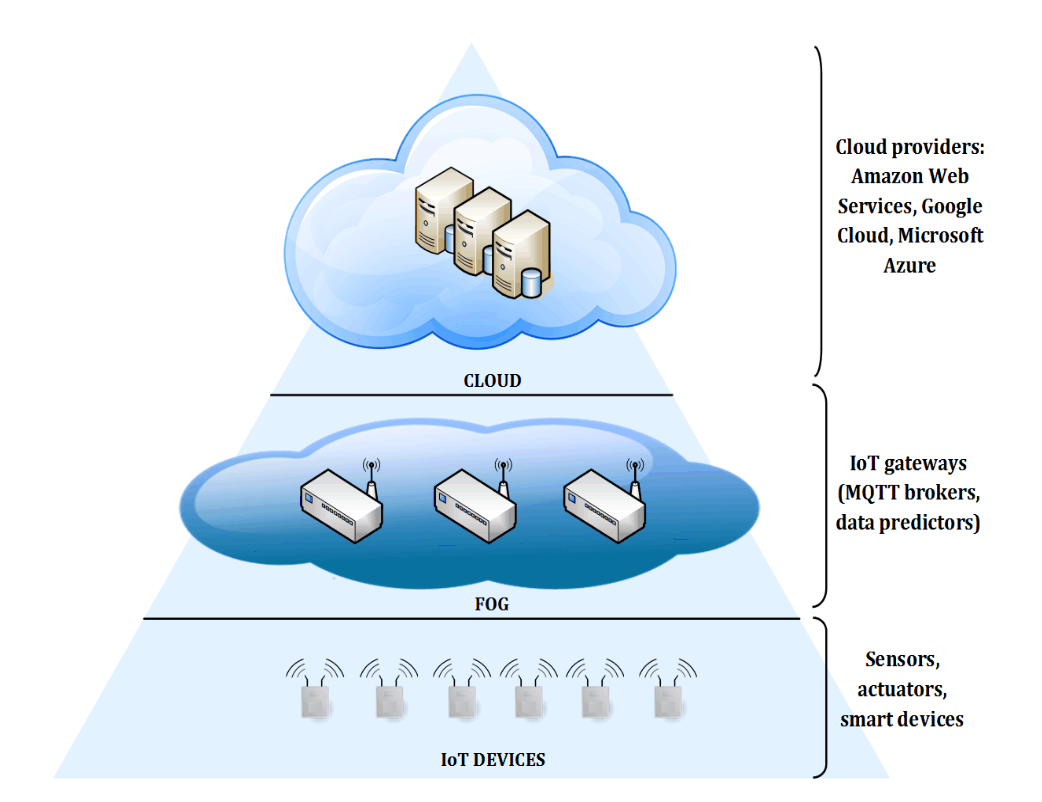
\includegraphics[scale=0.2]{eff_architecture.png}
	\caption{Introduced architecture for the integration of fog capabilities}
\end{figure}  

The way by which the devices at the different layers are exchanging data is using the MQTT-Protocol, where the nodes are the publishers and the fog layer, consisting of IoT-Gateways, represents the broker towards the cloud side. The means by which this proposed work is improving device energy consumption is by limiting the amount of data that has to be sent from the devices to the Gateways by applying a prediction algorithm using machine learning concepts at the fog layer. After an initial traning process, where sensed data from the devices is being sent to the fog layer, the fog layer is able to make forecasts for the data. Since the devices only have to transmit the data if the prediction fails to meet a predifined threshold, the amount of data transmitted by the devices can be greatly reduced. When using MQTT the QoS level impacts the enery consumption aswell. This effect can be seen in Fig. ???

\begin{figure}
	\centering
	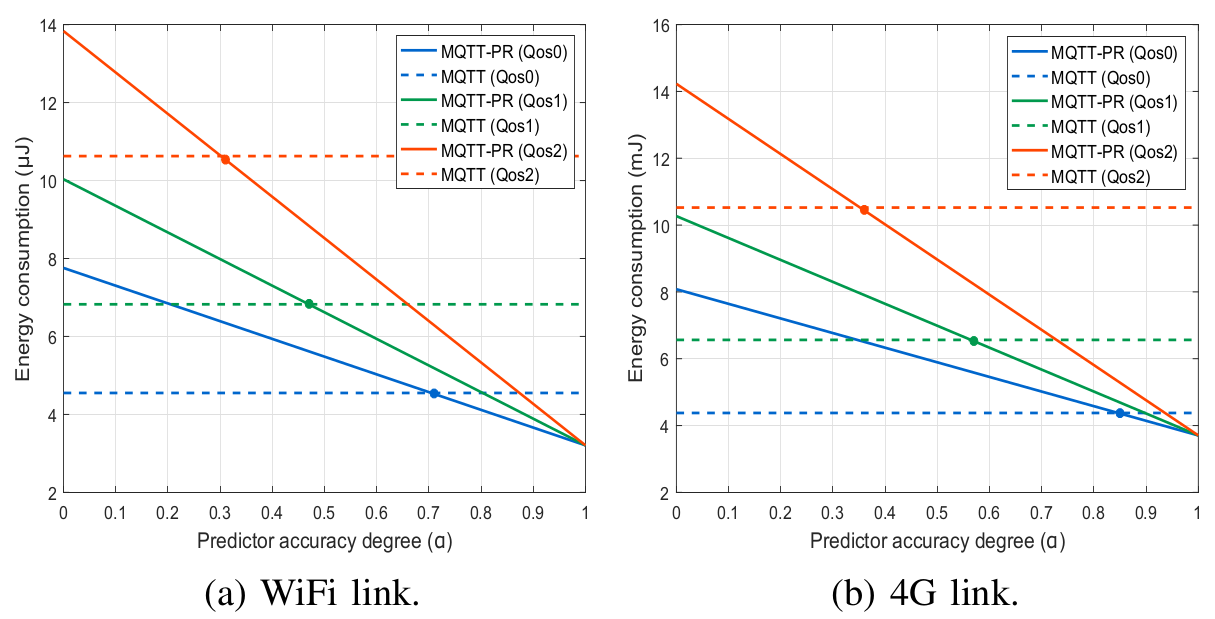
\includegraphics[scale=0.3]{comp_energy.png}
	\caption{Effect of different QoS levels on the energy consumption of the sensing devices}
\end{figure}

Another approach was introduced by Lin and Yang where the goal was to apply a cost effiecent deployment of fog computing into a logistics center use case. Similarely to above mentioned approach, they make the assumption that the implemented architecture  consists of the device layer, fog layer and a cloud layer. However they also add an additional edge layer that is placed at the very edge of the network, providing a intermediate layer between the devices and the fog layer and enabling up to real time decision making. This architecture follows the following workflow. The devices are sensing data at the shop floor and forward them to the edge layer, where decision making is applied depending on the location. If a decision cannot be made at the edge layer it is forwarded to the fog layer, where the responds time is lower than one second. The transmition of data towards the cloud in this framework only happens for long time storage. In order to implement an efficient workflow the edge and fog devices have to be placed efficiently to provide the fastest possible implementaion. 

